\section{Preliminary Work}

Prior research in computer networking hints that we should expect network configurations to share a common set of tokens. According to Hindle,\textit{et al.} 2012~\cite{naturalness}, regularities in bodies of texts can be easily exploited by NLP techniques. We took configurations from a large university network and split up each configuration file into a list of tokens. Tokens included all keywords and subnets with punctuation and newline characters stripped off. For every file we then plotted the percentage of tokens that exist in other router 
configuration files (Figure~\ref{fig:chart}).

\begin{figure}
	\centering
	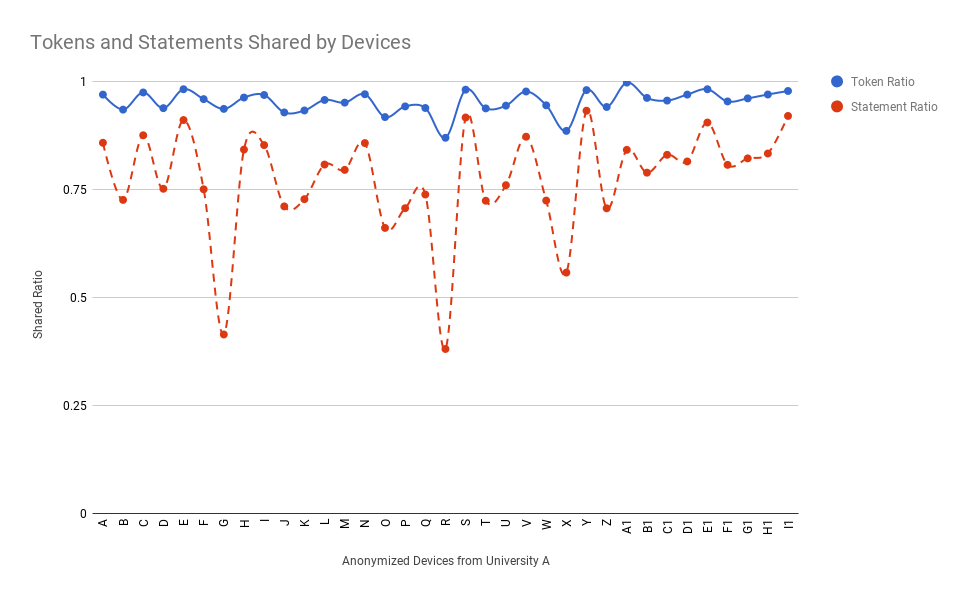
\includegraphics[width=\columnwidth]{chart.png}
	\caption{The plot shows how many tokens and statements a router configuration holds in common with the rest of the network. The data was taken from a large research university.}
    \label{fig:chart}
\end{figure}

Our results show that most of each file could be rebuilt from existing statements in routing configurations due to the amount of tokens they share. Given our results, and the observations made by~\cite{complexity} about how networks are configured, we can confidently hypothesize that most token suggestions can be generated from analyzing other existing configurations. This effectively makes all router configuration histories a part of the search space for our model. We use an N-gram model to generate predictions using likelihood estimators to score our n-grams. In particular, we made use of bigrams and trigrams, the latter of which performed consistently better.

We preprocessed the data and added placeholders for certain tokens like IP
addresses, subnet masks etc. This helped to reduce some noise and improved our
accuracies (Figure~\ref{fig:replacement_analysis}).
\begin{figure}
	\centering
	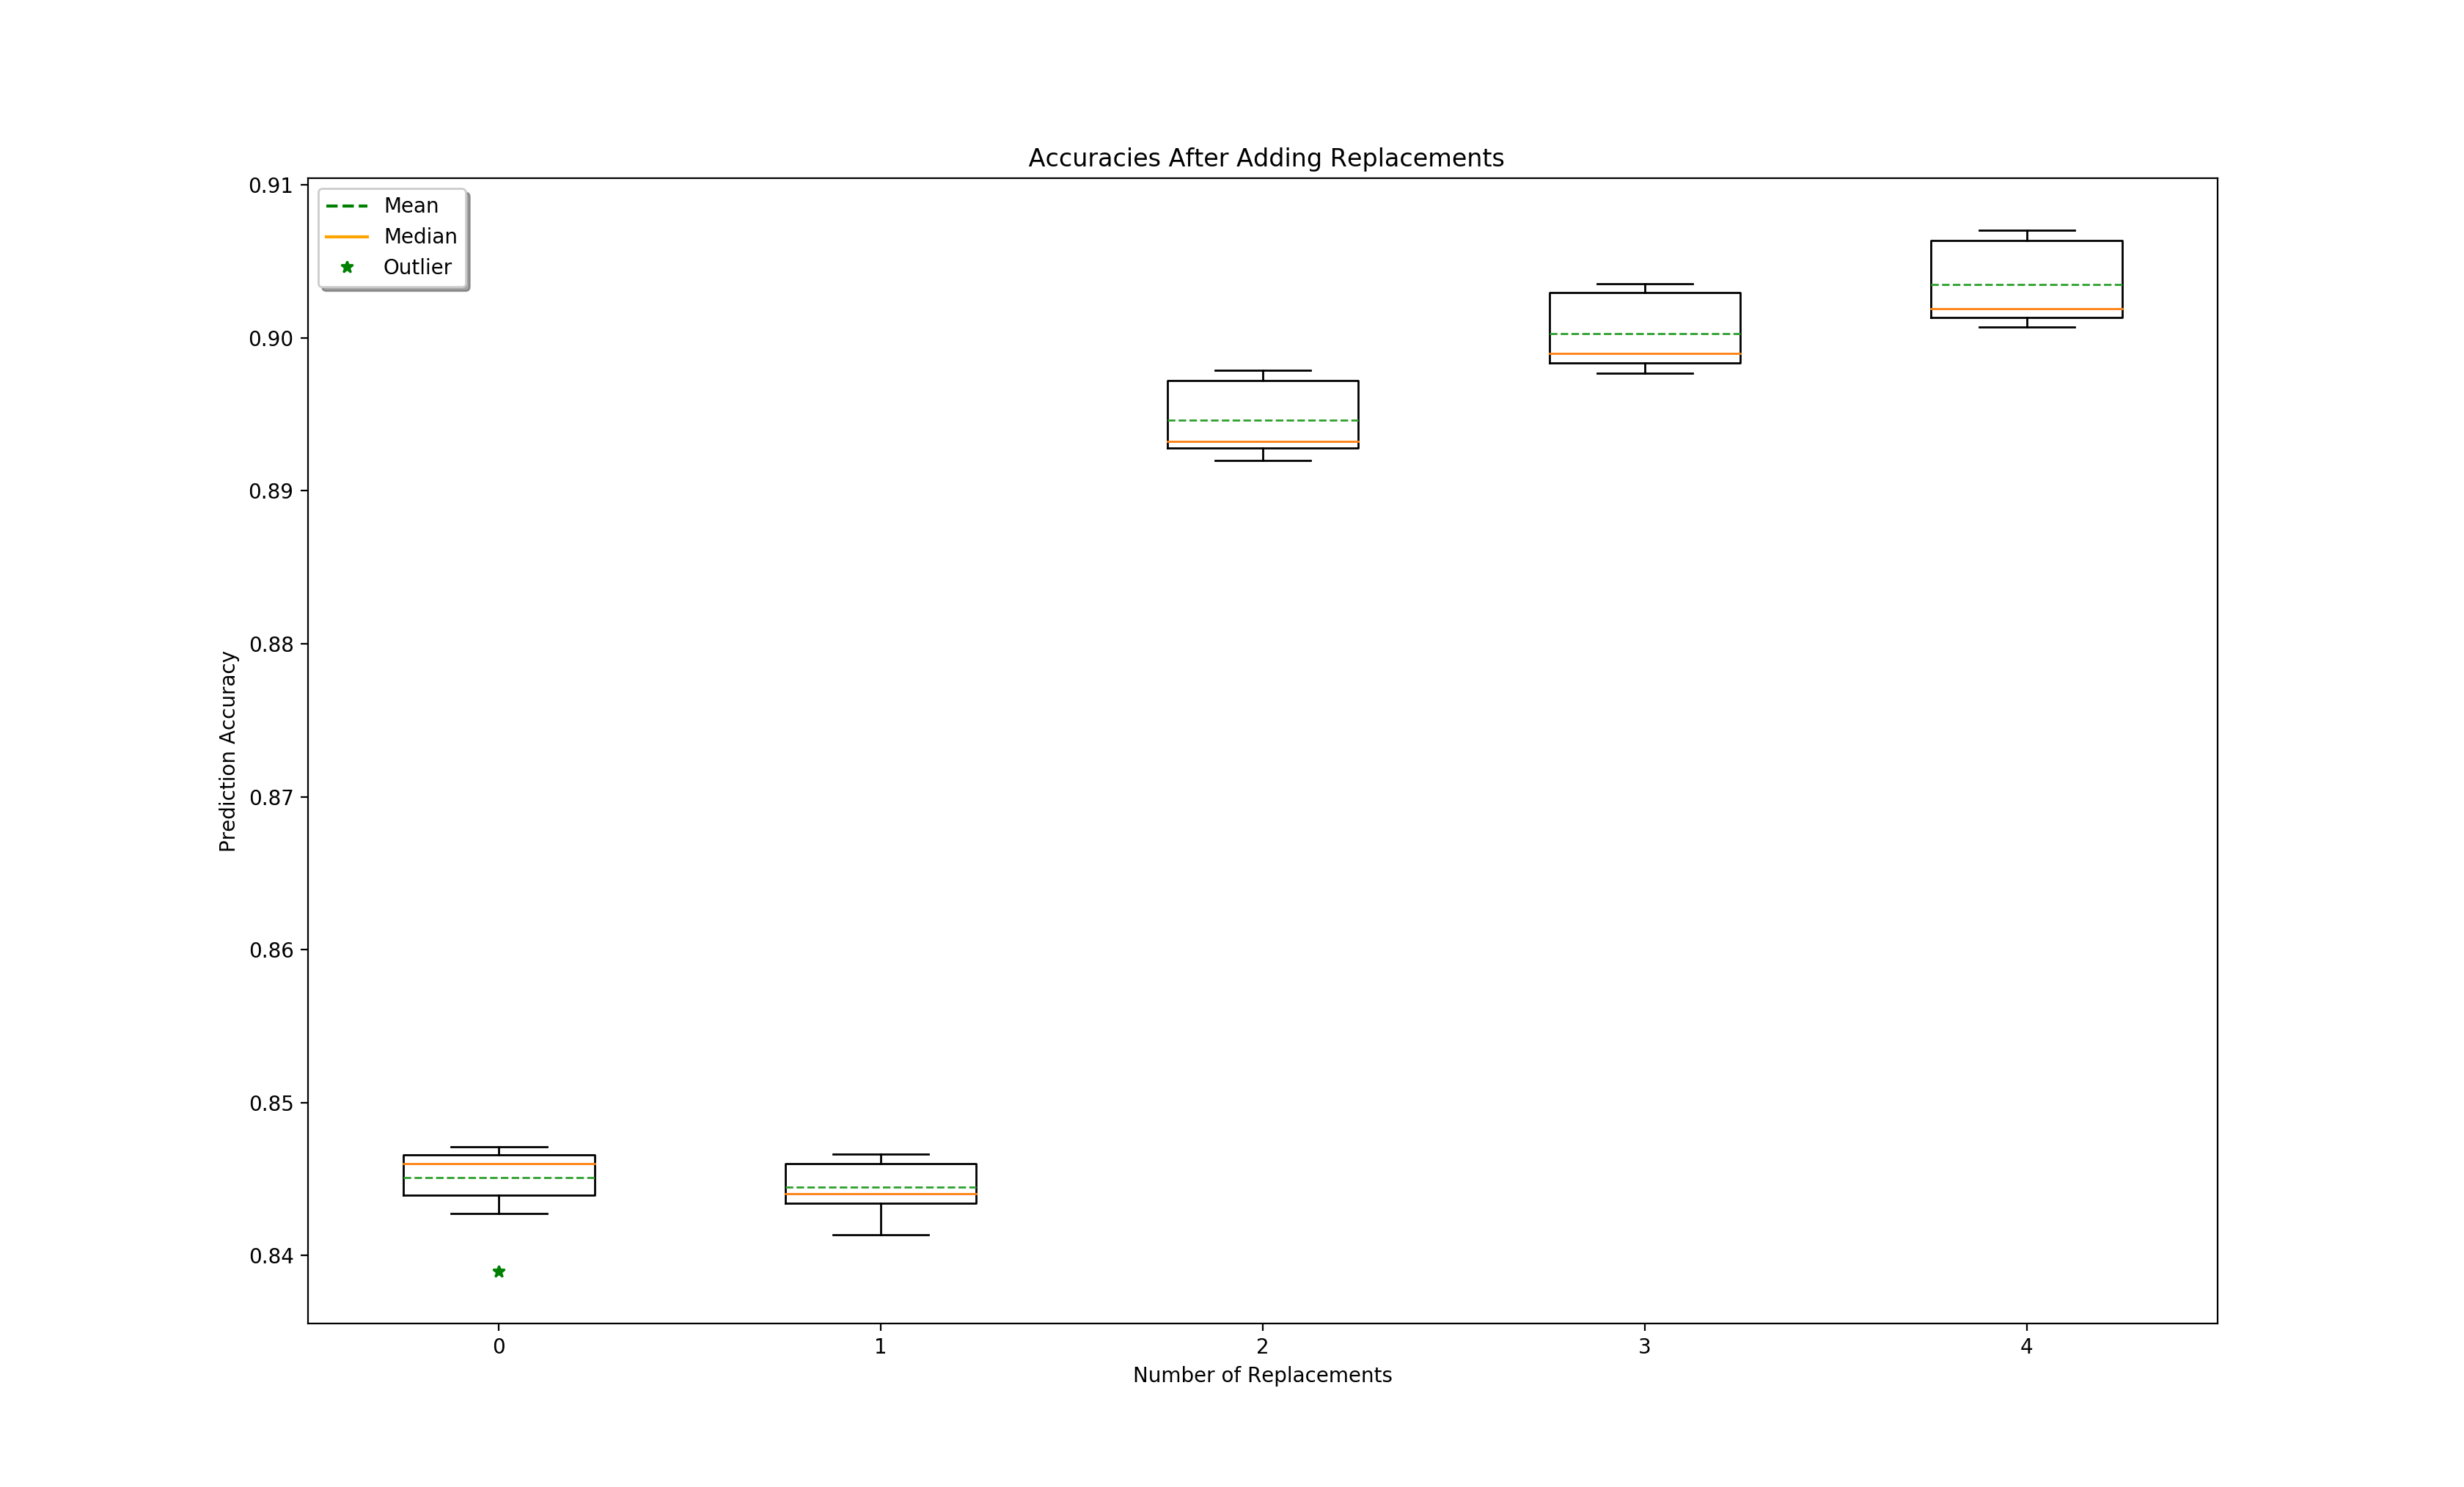
\includegraphics[width=\columnwidth]{replacement_analysis.png}
	\caption{Accuracy increase as we utilize placeholders for noisy tokens}
    \label{fig:replacement_analysis}
\end{figure}

\section{Results}

To test the accuracy of our model, we perform Leave One Out (LOO) Cross
Validation. This form of cross validation involves using one observation as
the validation set and the remaining observations as the training set. A
suggestion is marked as successful when the correct prediction lies within the
top three results generated by the model. We analyzed various large university
networks, varying sample sizes and number of devices
(Figure~\ref{fig:umn_analysis}).

\begin{figure}[H]
	\centering
	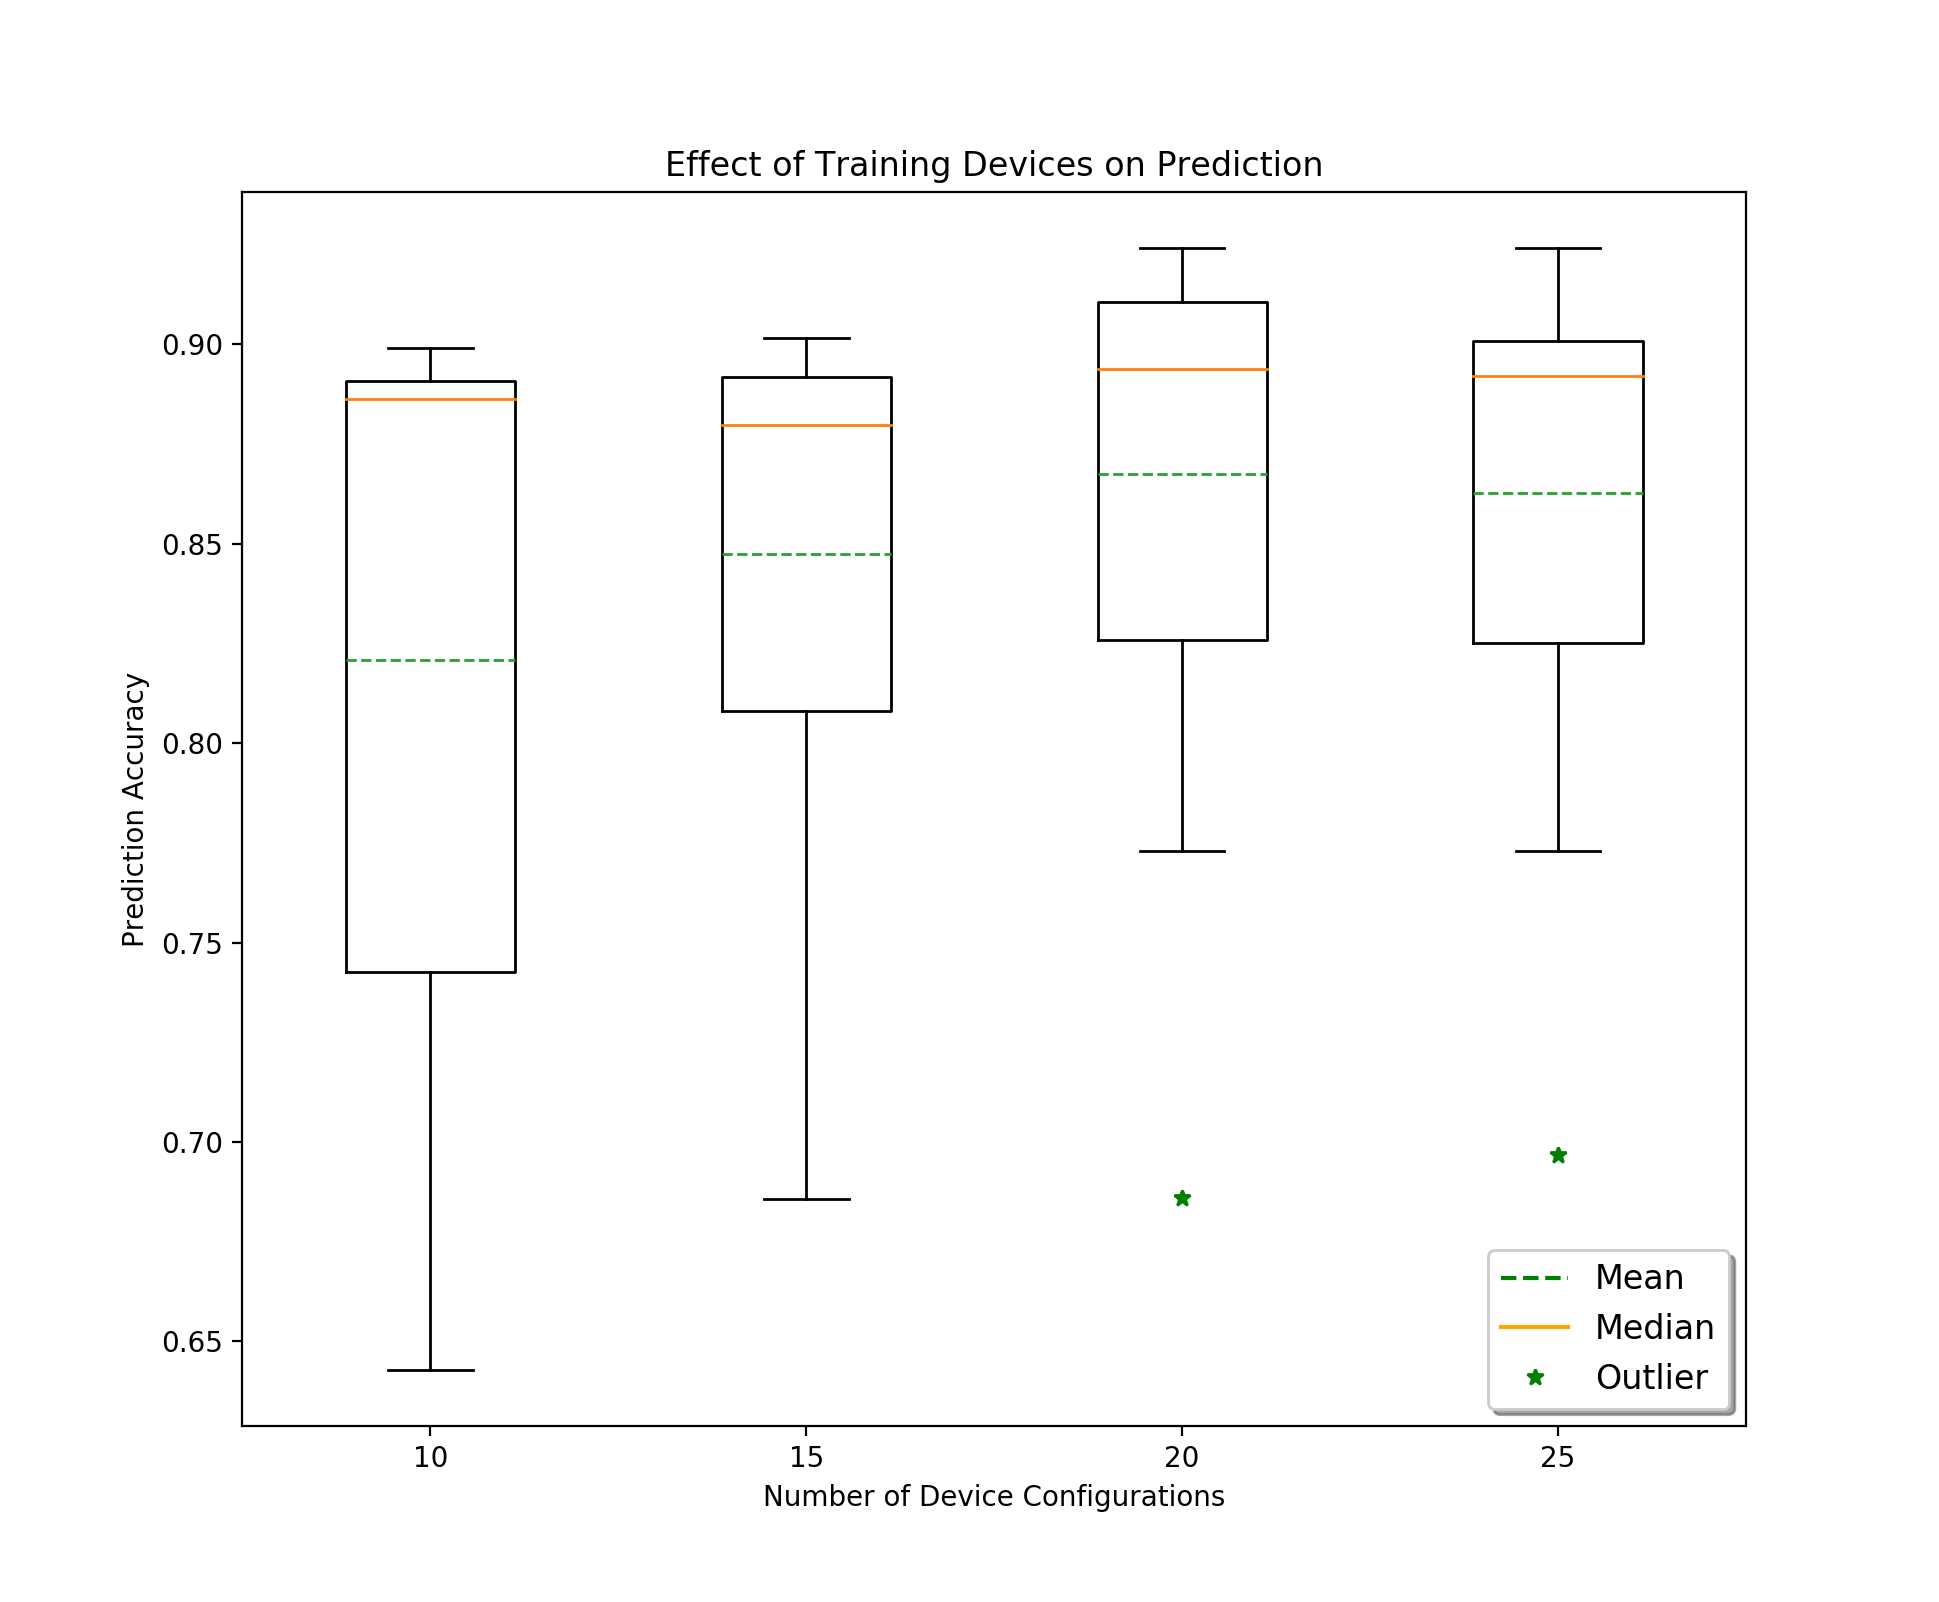
\includegraphics[width=\columnwidth]{umn_analysis.png}
	\caption{The bar charts show the accuracy of the model for each set of network configurations used as the validation set.}
    \label{fig:umn_analysis}
\end{figure}

*** ADD FIGURE WITH ALL 3 UNIVERSITIES ****

Our analyses help direct our attention towards areas of improvements for the model. The variance seen in our device analysis suggests that having different models for router of different "roles" could help improve prediction accuracies. Additionally, we plan on exploring the possibility of using larger n-grams to suggest complete statements. Lastly, we hope to evaluate our model against the current state of the art: tab-completion in CLIs on modern routers.
 
